\documentclass[11pt]{article}
\usepackage[a4paper,margin=1in]{geometry}
\usepackage{graphicx}
\usepackage{booktabs}
\usepackage{amsmath}
\usepackage{siunitx}
\usepackage{hyperref}
\usepackage{caption}
\usepackage{subcaption}
\usepackage{float}
\usepackage{array}
\usepackage{longtable}

\title{Modular Long-Context Sequence Modeling on WikiText-2}
\author{Krish Sachdev}
\date{3 June 2026}

\begin{document}
\maketitle

\begin{abstract}
I study long-context autoregressive language modeling on WikiText-2 using a modular decoder-only Transformer in which attention mechanisms, positional encodings, and local convolutional blocks can be swapped independently. Starting from a standard full-attention baseline at context length 1024, I evaluate 18 required final runs across attention variants, context lengths, positional extrapolation tests, and convolution-attention hybrids, then add the bonus Attention-Free Transformer (AFT) comparison as supplemental evidence. The selected baseline reaches a best/report validation perplexity of 65.02 at 1024 tokens. In the attention sweep, Sparse block at context 1024 gives the strongest validation perplexity (60.68), while the 4096-token sparse-block run remains the best long-context quality point among the tested efficient mechanisms (96.90 perplexity). Positional extrapolation favors ALiBi, which reaches PPL 83.73 at 2048 tokens after training at length 512. Among the AFT bonus variants, AFT-local is the strongest usable run at PPL 72.95, behind the best model by 14.15 perplexity points. The results show that theoretical attention efficiency is not enough on its own. The best model depends on measured perplexity, memory, throughput, and stability (under the Kaggle P100 training budget).
\end{abstract}

\section{Introduction}
Long-context language modeling is constrained by a direct systems problem. Standard causal self-attention compares every token with every previous token, so the attention score tensor grows quadratically in sequence length. For a small Transformer on WikiText-2, increasing context from 512 to 4096 sharply changes feasible batch size, GPU memory, and training throughput.~\cite{saidl2026}.

The implementation used here keeps the base language model fixed and swaps attention mechanism, positional encoding, and convolutional local-context modules. The experimental goal is to identify which choices improve validation perplexity. I report validation loss, perplexity, training throughput, inference throughput, peak GPU memory, gradient norms, finite-loss flags, virtual epoch timing, and W\&B run links for reproducibility.

\section{Background and Related Work}
\paragraph{Autoregressive Transformer language modeling.}
The baseline is a decoder-only Transformer trained with next-token cross entropy. Given validation loss $\ell$, perplexity is $\exp(\ell)$, so small loss differences are meaningful once the model is near convergence. Full causal self-attention is expensive because it materializes token-token interactions for every layer and head.

\paragraph{Efficient and structured attention.}
Sliding-window attention limits each token to a fixed local history. Sparse-block attention keeps attention structured around blocks, which can preserve more long-range information than a pure local window when the block pattern is useful. Grouped-query attention shares key-value projections across groups of query heads, reducing projection and cache cost while keeping more capacity than multi-query attention. In this implementation, the measured memory savings are modest because PyTorch masking and activation storage still dominate). This is to say the theoretical, asymptotic savings of sliding window and GQA were not fully explored in this implementation (it was discovered later in my implementation that these would require specialized kernels and more detailed optimization strategies, which I considered beyond the scope of analysis).

\paragraph{Attention-free sequence mixing.}
The bonus AFT runs replace explicit token-token attention with gating and learned position-dependent mixing inspired by Attention-Free Transformer models~\cite{zhai2021}. This is a useful counterpoint to sparse and grouped attention, since if and when the task can be solved with cheaper global mixing, AFT should approach the best attention variants in performance while reducing reliance on explicit attention matrices. I therefore compare the finished AFT-simple and AFT-local runs directly against the best model and against the successful 512 and 1024-token attention variants.

\paragraph{Positional encodings and extrapolation.}
Learned absolute embeddings are simple but tied to trained positions. RoPE rotates query/key features by position-dependent angles; ALiBi adds a linear distance bias directly to attention scores; learned relative positional encoding parameterizes token distance. The extrapolation experiment trains each method at length 512 and evaluates at 512, 1024, and 2048 to test whether the positional mechanism survives beyond the training context, per the assignment criteria.

\paragraph{Convolutional local bias.}
Convolutional modules add an explicit local n-gram bias. A pre-attention Conv1D block can reshape local representations before attention, while a gated convolutional FFN adds local filtering inside the feed-forward path. These hybrids may improve local syntax modeling, but they also add compute and can over-specialize if the extra module disrupts the Transformer optimization path.

\section{System Design and Implementation}
The model is a GPT-style decoder-only Transformer with vocabulary size 50,257, $d_{model}=384$, six layers, six heads, dropout 0.1, and a feed-forward multiplier of four. Hydra config groups control the model, data, trainer, positional encoding, and convolutional block. The code path uses GPT-style small-normal initialization for linear and embedding weights, AdamW optimization, cosine learning-rate decay with warmup, automatic mixed precision, gradient clipping, and checkpointed resume.

\begin{table}[H]
\centering
\caption{Implementation components used in the final Core ML suite.}
\label{tab:system-components}
\resizebox{\textwidth}{!}{%
\begin{tabular}{llll}
\toprule
Component & Choices in final report & Main source & Purpose \\
\midrule
Attention & full, sliding window, sparse block, GQA, AFT bonus & \texttt{core\_ml/src/attention.py} & long-context mechanism \\
Position & absolute, RoPE, ALiBi, relative & \texttt{core\_ml/src/positional.py} & position and extrapolation \\
Convolution & none, pre-attention, gated FFN & \texttt{core\_ml/src/model.py} & local-context inductive bias \\
Training & AdamW, AMP, cosine LR, checkpoints & \texttt{core\_ml/src/train.py} & controlled optimization \\
Reporting & W\&B plus CSV/LaTeX assets & \texttt{core\_ml/report} & reproducibility \\
\bottomrule
\end{tabular}
}
\end{table}

\section{Experimental Setup}
All selected Core ML runs use WikiText-2 raw text with the GPT-2 tokenizer, maximum model sequence length 4096, validation token cap 300,000, full train tokens enabled, evaluation every 500 steps, 40 validation batches, and 12,000 maximum training steps. The optimizer is AdamW with learning rate $3\times10^{-4}$, weight decay 0.01, 500 warmup steps, cosine decay, AMP enabled on CUDA, and gradient clipping at 1.0. Context-dependent batch sizes are 8 at length 512, 4 at length 1024, 2 at length 2048, and 1 at length 4096.

The W\&B export contains 31 recent finished final runs and 202 total historical project runs; 18 required, successfully-finished runs are selected for the main required comparison. Failed linear-attention runs are excluded from the required comparison because the assignment requires three attention variants, which are satisfied by sliding-window, sparse-block, and GQA runs. AFT is handled separately as a bonus comparison: AFT-simple and AFT-local have usable finished metrics, while the latest finished AFT-full run still has no usable validation metric.

Because training is step-based rather than epoch-based, I report a virtual epoch time: approximately $2.43$M WikiText-2 training tokens divided by measured training tokens/sec. This gives an epoch-equivalent timing signal without pretending the loader is organized as a classical epoch loop.

\subsection{Parameter Choices and Rationale}
The setup parameters were fixed to make the comparisons controlled rather than to tune each architecture separately. WikiText-2 raw text and the GPT-2 tokenizer keep the task small enough for repeated Kaggle runs while still using a realistic subword vocabulary. The maximum model sequence length is 4096 because the assignment focuses on long-context behavior, while the validation token cap and 40 validation batches keep evaluation frequent enough to catch instability without consuming the whole GPU budget.

The 12,000-step training budget is a compute compromise. It is long enough for the small model to separate attention mechanisms and positional encodings, but short enough to run the full required suite, reruns, and bonus attempts. The learning rate $3\times10^{-4}$, AdamW, weight decay 0.01, 500 warmup steps, cosine decay, AMP, and gradient clipping at 1.0 were kept constant so that differences in perplexity are mainly attributable to the architecture choices rather than per-run optimizer tuning. The context-dependent batch sizes are capacity controls: longer contexts require smaller batches to fit on the available GPU, so throughput and memory are reported alongside perplexity instead of treating all context lengths as equally cheap.

\begin{table}[H]
\centering
\small
\caption{Assignment requirements mapped to selected final experiments.}
\label{tab:coverage}
\resizebox{\textwidth}{!}{%
\begin{tabular}{llll}
\toprule
Part & Requirement & Status & Report PPL \\
\midrule
Part 1 & Baseline full-attention Transformer at context 1024 & Complete & 65.02 \\
Part 2 & Sliding-window attention at context 512 & Complete & 64.13 \\
Part 2 & Sliding-window attention at context 1024 & Complete & 70.53 \\
Part 2 & Sliding-window attention at context 2048 & Complete & 122.86 \\
Part 2 & Sliding-window attention at context 4096 & Complete & 153.59 \\
Part 2 & Sparse-block attention at context 512 & Complete & 69.08 \\
Part 2 & Sparse-block attention at context 1024 & Complete & 60.68 \\
Part 2 & Sparse-block attention at context 2048 & Complete & 79.09 \\
Part 2 & Sparse-block attention at context 4096 & Complete & 96.90 \\
Part 2 & Grouped-query attention at context 512 & Complete & 62.70 \\
Part 2 & Grouped-query attention at context 1024 & Complete & 65.77 \\
Part 2 & Grouped-query attention at context 2048 & Complete & 109.70 \\
Part 2 & Grouped-query attention at context 4096 & Complete & 149.98 \\
Part 3 & RoPE trained at context 512 with extrapolation eval & Complete & 59.09 \\
Part 3 & ALiBi trained at context 512 with extrapolation eval & Complete & 58.80 \\
Part 3 & Relative positional encoding trained at context 512 with extrapolation eval & Complete & 61.70 \\
Part 4 & Pre-attention Conv1D hybrid with GQA and RoPE & Complete & 63.23 \\
Part 4 & Gated convolutional FFN hybrid with GQA and RoPE & Complete & 71.70 \\
Bonus & AFT-simple at context 512 & Complete supplemental run & 74.61 \\
Bonus & AFT-local at context 512 & Complete supplemental run & 72.95 \\
Bonus & AFT-full at context 512 & Attempted; no usable finished metric & -- \\
\bottomrule
\end{tabular}
}
\end{table}

\section{Results}
\subsection{Part 1: Baseline Transformer}
The full-attention baseline at context 1024 is the reference point for the rest of the report. It reaches best/report validation loss 4.1747 and perplexity 65.02, with peak memory 4.14 GB and inference throughput 72665 tokens/sec.

\begin{table}[H]
\centering
\small
\caption{Baseline Transformer metrics.}
\label{tab:baseline}
\resizebox{\textwidth}{!}{%
\begin{tabular}{lrrrrrrrrr}
\toprule
Model & Context & Batch & Steps & Best/Report step & Best/Report val loss & Best/Report val PPL & Train tok/s & Infer tok/s & Peak mem GB \\
\midrule
Full attention + learned absolute positions & 1024 & 4 & 12000 & 12000 & 4.17 & 65.02 & 20993.00 & 72665.00 & 4.14 \\
\bottomrule
\end{tabular}
}
\end{table}

\subsection{Part 2: Attention Variants Across Context Length}
Table~\ref{tab:attention-quality} compares validation perplexity across context length. The strongest attention-sweep result is Sparse block at context 1024, with best/report perplexity 60.68. At the longest tested length, sparse block is the best quality point with perplexity 96.90; this is substantially better than GQA and sliding window at 4096 in this run set.

\begin{table}[H]
\centering
\small
\caption{Attention validation perplexity across context length. Lower is better.}
\label{tab:attention-quality}
\resizebox{\textwidth}{!}{%
\begin{tabular}{lrrrr}
\toprule
Attention & 512 & 1024 & 2048 & 4096 \\
\midrule
Sliding window & 64.13 & 70.53 & 122.86 & 153.59 \\
Sparse block & 69.08 & 60.68 & 79.09 & 96.90 \\
GQA & 62.70 & 65.77 & 109.70 & 149.98 \\
\bottomrule
\end{tabular}
}
\end{table}

\begin{table}[H]
\centering
\small
\caption{Attention efficiency and stability metrics.}
\label{tab:attention-efficiency}
\resizebox{\textwidth}{!}{%
\begin{tabular}{lrrrrrr}
\toprule
Attention & Context & Best/Report val PPL & Peak mem GB & Train tok/s & Infer tok/s & Grad norm \\
\midrule
GQA & 512 & 62.70 & 3.63 & 24729.00 & 87972.00 & 1.56 \\
Sliding window & 512 & 64.13 & 3.65 & 23992.00 & 85152.00 & 1.52 \\
Sparse block & 512 & 69.08 & 3.65 & 24081.00 & 84865.00 & 1.53 \\
GQA & 1024 & 65.77 & 4.12 & 21180.00 & 73944.00 & 1.60 \\
Sliding window & 1024 & 70.53 & 4.14 & 20706.00 & 71562.00 & 1.44 \\
Sparse block & 1024 & 60.68 & 4.14 & 20790.00 & 71577.00 & 1.55 \\
GQA & 2048 & 109.70 & 5.13 & 16265.00 & 52890.00 & 1.62 \\
Sliding window & 2048 & 122.86 & 5.15 & 15912.00 & 50963.00 & 1.33 \\
Sparse block & 2048 & 79.09 & 5.15 & 15921.00 & 51115.00 & 1.52 \\
GQA & 4096 & 149.98 & 7.17 & 11503.00 & 36902.00 & 1.39 \\
Sliding window & 4096 & 153.59 & 7.19 & 11181.00 & 33952.00 & 1.23 \\
Sparse block & 4096 & 96.90 & 7.18 & 11234.00 & 34745.00 & 1.49 \\
\bottomrule
\end{tabular}
}
\end{table}

It needs mentioning again that for a fixed context, sliding-window and sparse-block attention do not obtain large memory reductions because the PyTorch implementation still works with dense masks and dense activations  (no custom memory-efficient kernels were used).

\paragraph{Why the theoretical savings are muted here.}
The efficient-attention variants reduce which token pairs are logically allowed to interact, but the implementation still stores normal Transformer activations and uses PyTorch masking rather than a custom block-sparse or fused local-attention kernel. Therefore the memory profile is still dominated by hidden states, projections, residual activations, and dense intermediate tensors. This is not a correctness problem for the assignment comparison, because the reported metrics are measured from the actual implementation, but it does limit the strength of any claim about asymptotic efficiency. The practical conclusion is that sparse patterns and GQA should be judged here by measured perplexity, throughput, and peak memory, not by theoretical complexity alone.


\subsection{Part 3: Positional Encoding Extrapolation}
All three positional encodings are trained at length 512 and evaluated at 512, 1024, and 2048. RoPE has strong in-distribution validation perplexity, but its 2048-token extrapolation degrades sharply in this small-model setting. ALiBi gives the best 2048-token extrapolation among the three, with PPL 83.73. Relative position encoding is close to ALiBi at 2048 but slightly worse in the selected run.

\begin{table}[H]
\centering
\small
\caption{Positional extrapolation from train length 512.}
\label{tab:positional}
\resizebox{\textwidth}{!}{%
\begin{tabular}{lrrrrrrr}
\toprule
Positional encoding & Train length & Best/Report val PPL & PPL @512 & PPL @1024 & PPL @2048 & Inflation 1024/512 & Inflation 2048/512 \\
\midrule
ALiBi & 512 & 58.80 & 68.12 & 60.76 & 83.73 & 0.89 & 1.23 \\
Relative & 512 & 61.70 & 71.95 & 62.10 & 84.71 & 0.86 & 1.18 \\
RoPE & 512 & 59.09 & 64.00 & 71.62 & 145.33 & 1.12 & 2.27 \\
\bottomrule
\end{tabular}
}
\end{table}

\subsection{Part 4: Convolution and Attention Hybrids}
The convolutional hybrids use GQA and RoPE. The closest non-conv reference available in the final required suite is GQA with absolute positions at context 1024, so its important to mention that the comparison is useful but not a perfect ablation of convolution alone. Pre-attention convolution is the better hybrid, with best/report perplexity 63.23; gated convolutional FFN is less attractive because its best checkpoint is worse and its final validation perplexity is much higher (likely instability).

\begin{table}[H]
\centering
\small
\caption{Convolutional hybrid comparison against closest GQA non-conv reference.}
\label{tab:conv}
\resizebox{\textwidth}{!}{%
\begin{tabular}{lrrrrrrrr}
\toprule
Model & Attention & Position & Conv & Best/Report val PPL & Delta PPL vs GQA ref & Peak mem GB & Train tok/s & Infer tok/s \\
\midrule
Reference GQA non-conv & gqa & absolute & none & 65.77 & 0.00 & 4.12 & 21180.00 & 73944.00 \\
Pre Attention & gqa & rope & pre\_attention & 63.23 & -2.53 & 4.24 & 17848.00 & 63133.00 \\
Gated Ffn & gqa & rope & gated\_ffn & 71.70 & 5.94 & 4.67 & 11313.00 & 43453.00 \\
\bottomrule
\end{tabular}
}
\end{table}

\section{Cross-Experiment Analysis}
I observed that quality and efficiency do not rank architectures in the same order. Sparse-block attention provides the best attention-sweep perplexity, especially at 1024 and 4096, but its measured memory is not meaningfully below the other masked attention variants at the same context (as explained earlier). GQA is attractive for inference throughput at short context, reaching 87972 tokens/sec at context 512, but it does not dominate validation perplexity at longer contexts (instability hurts final ppl numbers). Sliding window is simple and stable, but its local-only constraint hurts quality at 2048 and 4096.

Regarding positional results, ALiBi and relative encoding both remain near the low-80s perplexity range at 2048. Their 1024-token perplexity is lower than their 512-token extrapolation pass, which I treated as evidence of robustness rather than a literal claim that longer context is intrinsically easier, since the validation chunks differ by evaluation length. RoPE, despite strong 512-token quality, rises to PPL 145.33 at 2048. In this setup, ALiBi is the best extrapolation choice.

\begin{table}[H]
\centering
\small
\caption{Final decision table.}
\label{tab:winners}
\resizebox{\textwidth}{!}{%
\begin{tabular}{lrrr}
\toprule
Decision criterion & Winner & Evidence & Caveat \\
\midrule
Lowest attention-sweep perplexity & Sparse block ctx 1024 & PPL 60.68 & Step-budget result; batch size changes with context. \\
Best memory efficiency in attention sweep & GQA ctx 512 & Peak 3.63 GB & Memory is not normalized across context lengths. \\
Best inference throughput in attention sweep & GQA ctx 512 & 87972 tokens/s & Shorter contexts naturally benchmark faster. \\
Best 2048-token extrapolation & ALiBi & PPL @2048 83.73 & All positional runs trained at context 512. \\
Best convolutional hybrid & Pre Attention & PPL 63.23 & Compared against closest non-conv GQA reference, not an exact GQA+RoPE ablation. \\
\bottomrule
\end{tabular}
}
\end{table}

\begin{figure}[H]
\centering
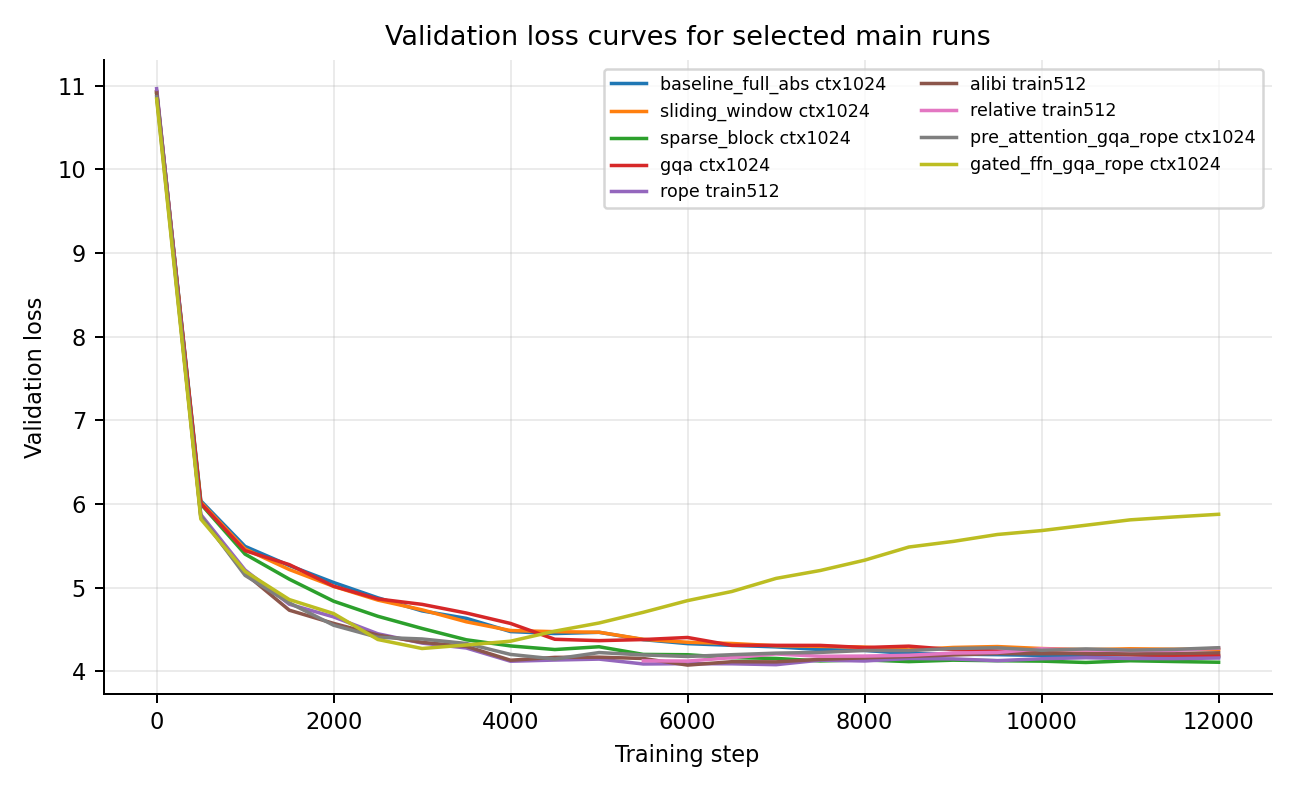
\includegraphics[width=0.92\textwidth]{figures/main_val_loss_curves.png}
\caption{Validation loss curves for representative main runs.}
\label{fig:loss-curves}
\end{figure}
\begin{figure}[H]
\centering
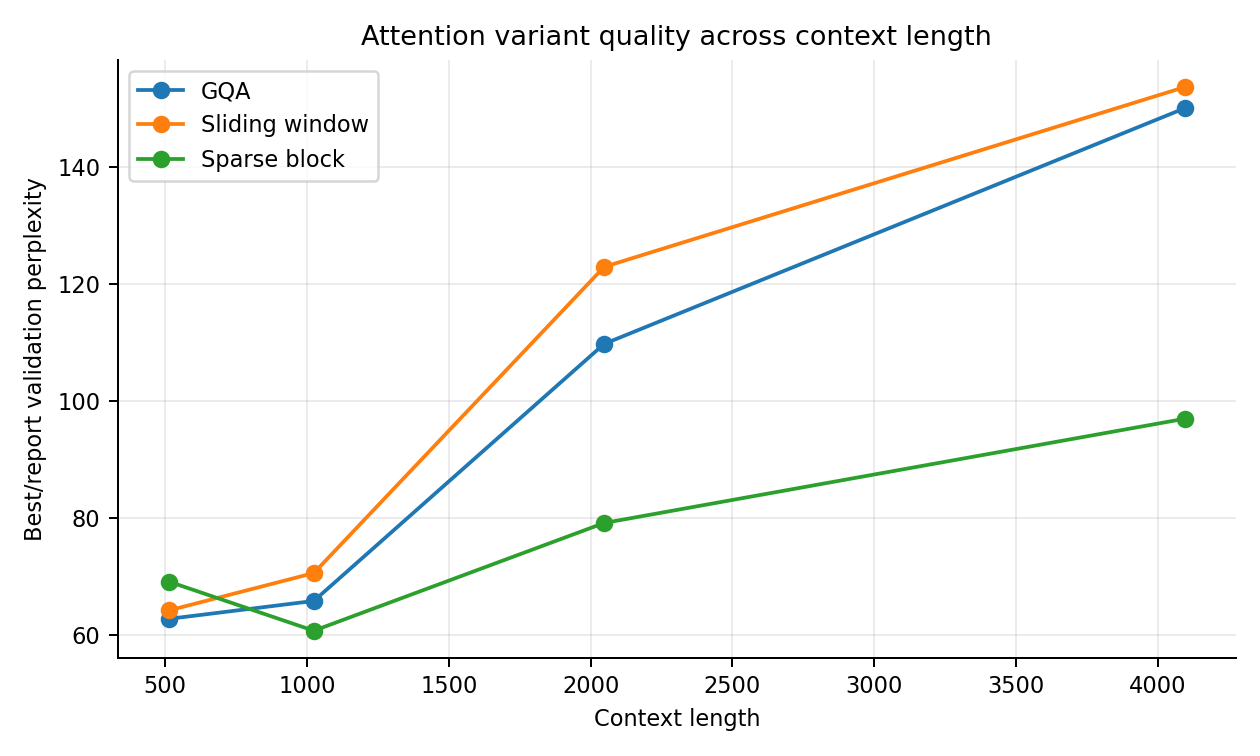
\includegraphics[width=0.92\textwidth]{figures/attention_ppl_vs_context.png}
\caption{Best/report validation perplexity for attention variants across context lengths.}
\label{fig:attn-ppl-context}
\end{figure}
\begin{figure}[H]
\centering
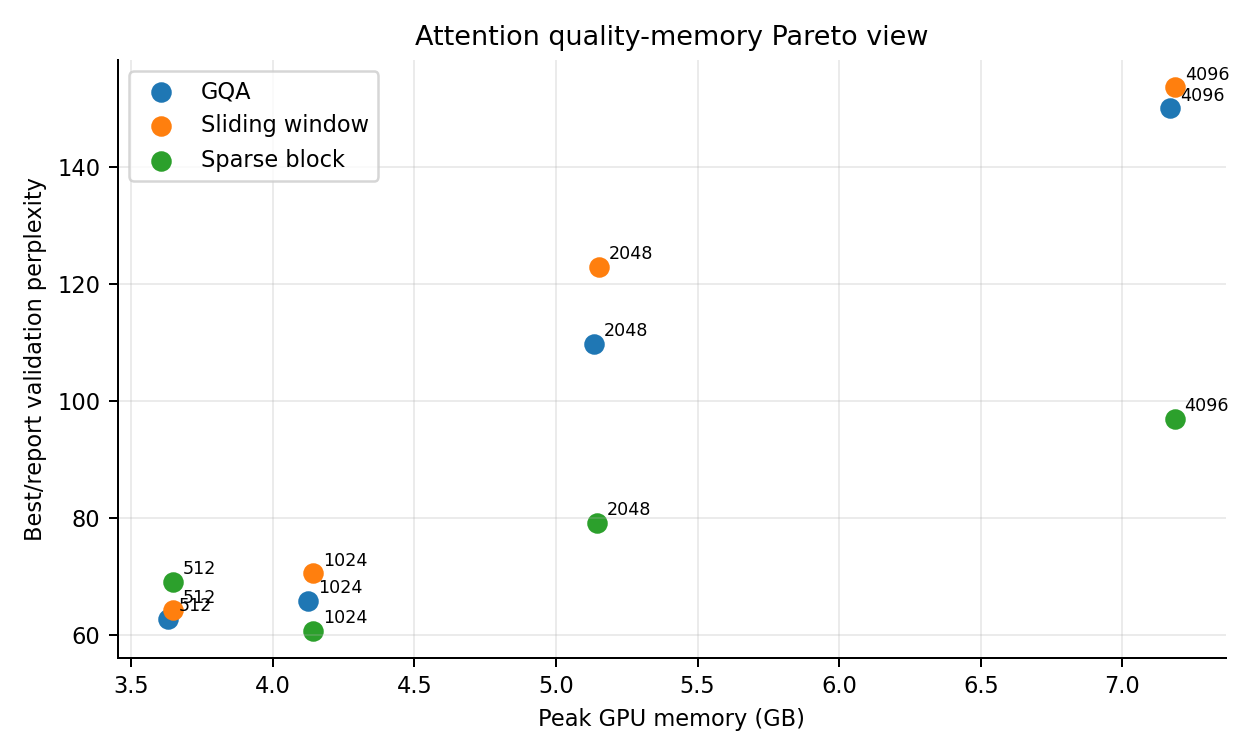
\includegraphics[width=0.92\textwidth]{figures/attention_pareto_memory_ppl.png}
\caption{Attention quality-memory tradeoff. Labels mark context length.}
\label{fig:attn-pareto}
\end{figure}
\begin{figure}[H]
\centering
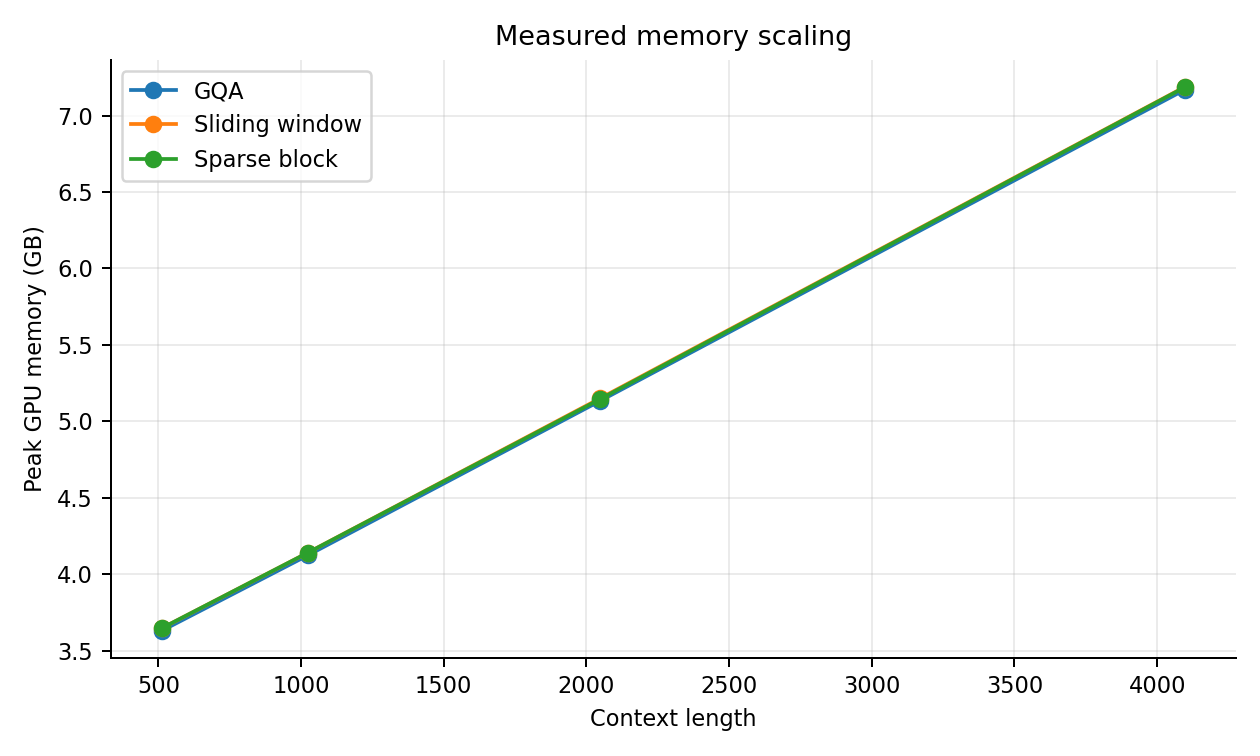
\includegraphics[width=0.92\textwidth]{figures/memory_vs_context.png}
\caption{Measured peak GPU memory as context length increases.}
\label{fig:memory-context}
\end{figure}
\begin{figure}[H]
\centering
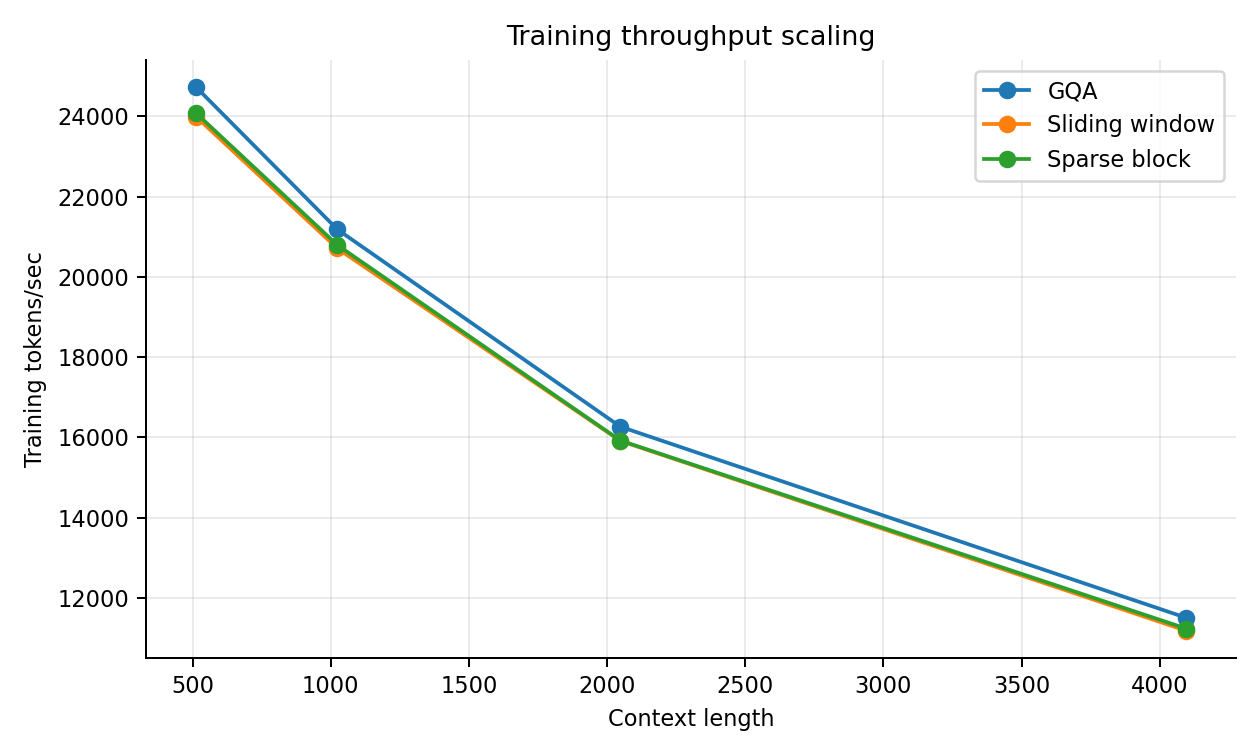
\includegraphics[width=0.92\textwidth]{figures/throughput_vs_context.png}
\caption{Training throughput as context length increases.}
\label{fig:throughput-context}
\end{figure}
\begin{figure}[H]
\centering
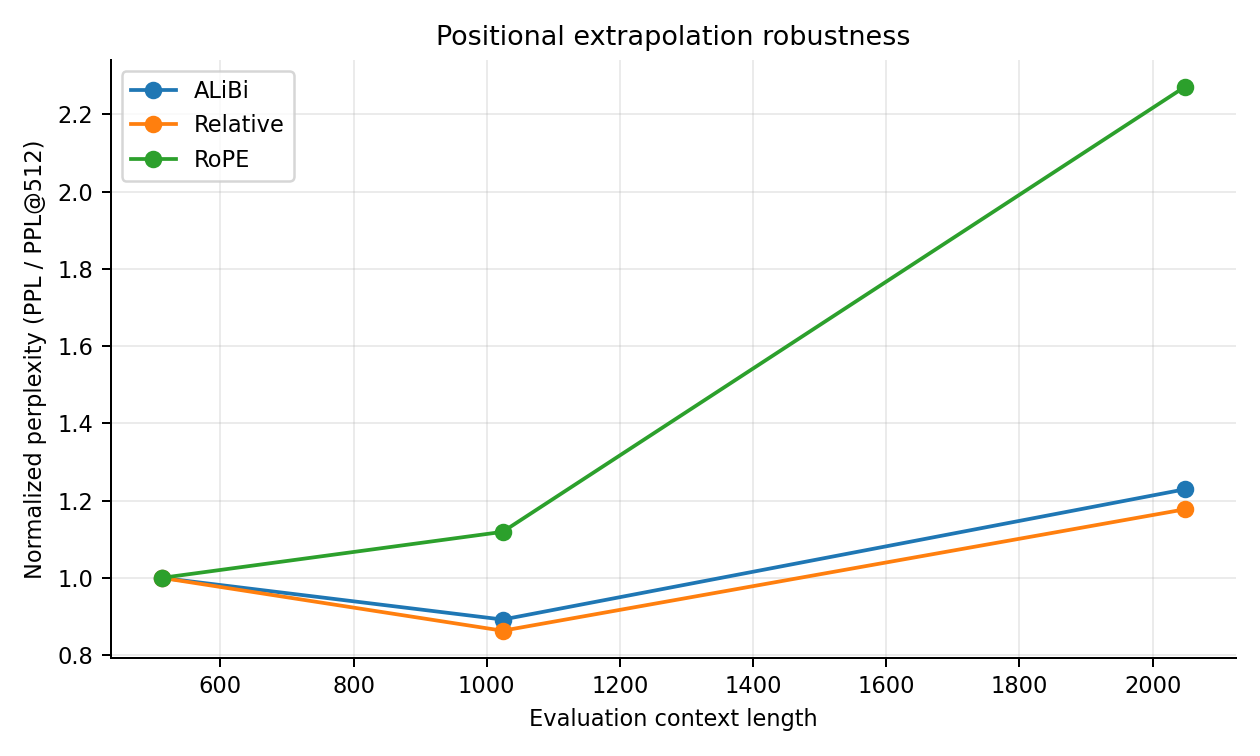
\includegraphics[width=0.92\textwidth]{figures/positional_extrapolation.png}
\caption{Normalized perplexity inflation when evaluating beyond the 512-token training length.}
\label{fig:pos-extrap}
\end{figure}
\begin{figure}[H]
\centering
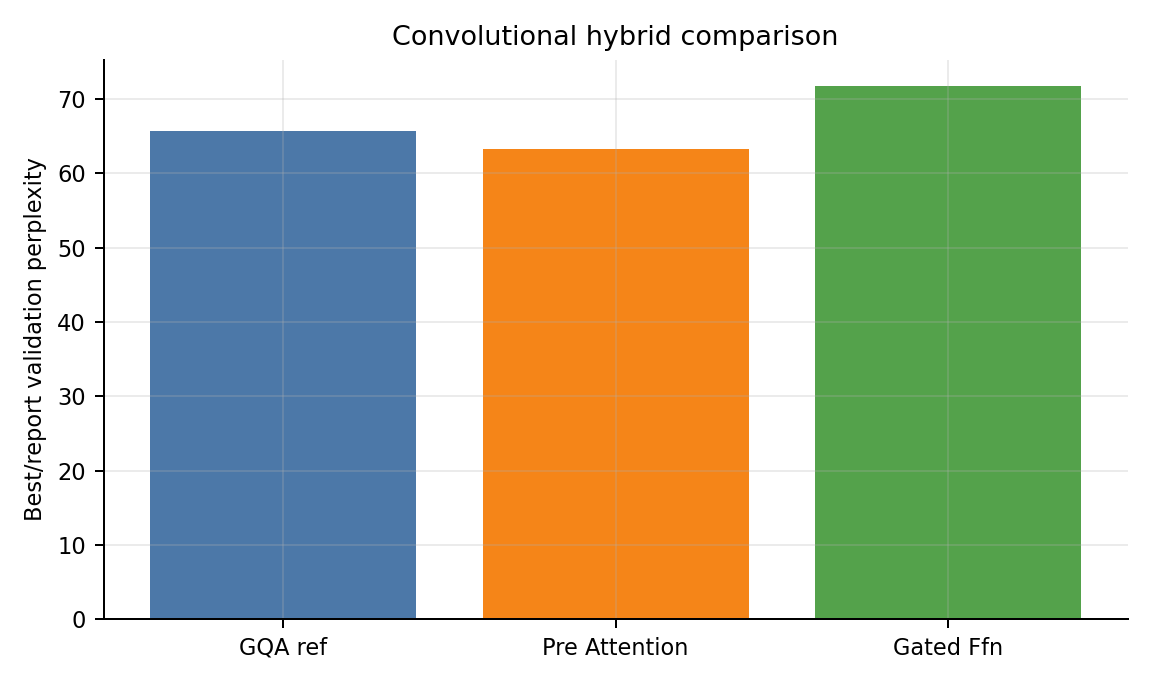
\includegraphics[width=0.92\textwidth]{figures/conv_hybrid_ppl.png}
\caption{Validation perplexity comparison for convolutional hybrids.}
\label{fig:conv}
\end{figure}

\section{Bonus: Attention-Free Transformer}
The bonus section of the assignment asks for variants from the Attention-Free Transformer paper and a comparison with the best previous model. I ran AFT-simple, AFT-local, and AFT-full at context length 512. For fairness, I keep the AFT results separate from the required-suite claims and compare only the newest finished run for each AFT experiment name. The current W\&B export shows usable finished metrics for AFT-simple and AFT-local. The latest finished AFT-full row exists but contains no validation loss or perplexity, so I do not count it as a successful metric result.

\begin{table}[H]
\centering
\small
\caption{Bonus AFT comparison against the best required Core ML result. Lower perplexity is better.}
\label{tab:aft-bonus}
\resizebox{\textwidth}{!}{%
\begin{tabular}{llrrrr}
\toprule
Model & Run & Report step & Val loss & Val PPL & Delta PPL vs best required \\
\midrule
Best required result & \texttt{coreml\_p3\_alibi\_train512} & 6000 & 4.074 & 58.80 & 0.00 \\
AFT-local & \texttt{coreml\_bonus\_aft\_local\_ctx512} & 12000 & 4.290 & 72.95 & +14.15 \\
AFT-simple & \texttt{coreml\_bonus\_aft\_simple\_ctx512} & 12000 & 4.312 & 74.61 & +15.80 \\
AFT-full & \texttt{coreml\_bonus\_aft\_full\_ctx512} & -- & -- & -- & -- \\
\bottomrule
\end{tabular}
}
\end{table}

\begin{figure}[H]
\centering
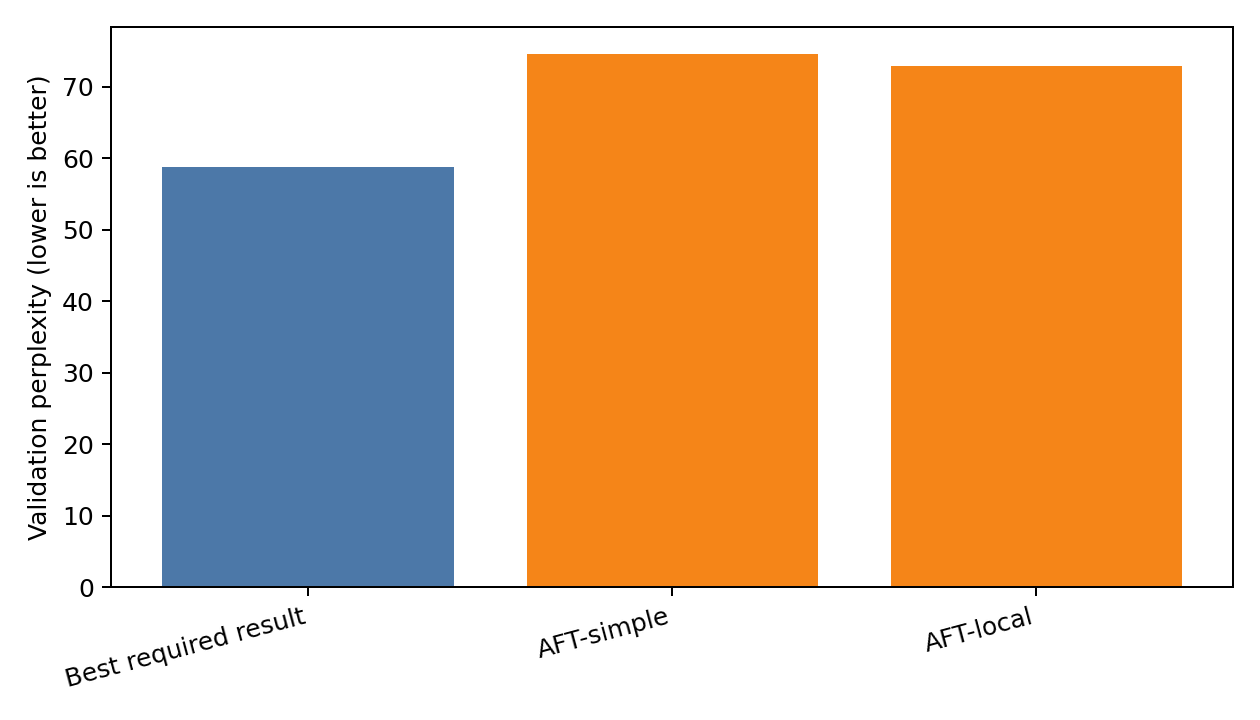
\includegraphics[width=0.82\textwidth]{figures/core_bonus_aft_vs_required.png}
\caption{Validation perplexity for the usable AFT bonus runs compared with the best required model.}
\label{fig:aft-bonus}
\end{figure}

Without getting too granular, AFT-local is the best AFT result, improving on AFT-simple by 1.65 perplexity points. It still trails the best required run, ALiBi trained at length 512, by 14.15 perplexity points. Against the successful 512-token attention variants, AFT-local also remains behind GQA (62.70), sliding-window attention (64.13), and sparse block attention (69.08). The gap is smaller against sparse block than against GQA, but the direction is consistent: in this implementation and under the 12k-step budget, the attention-free mixer did not replace explicit attention as the strongest quality choice. Though according to the \texttt{val\_loss} curves, it may have benefited from longer tuning.

AFT-local and AFT-simple still provide useful evidence: both train to finite validation losses and land in the same broad quality range as the weaker long-context attention runs. The result suggests that the AFT path is viable enough for experimentation, but it needs more tuning before it can be presented as a better substitute for the required attention variants. The most likely next changes would be a longer tuning run, a careful learning-rate and dropout sweep, and a more optimized implementation of the AFT-full variant.

\paragraph{AFT-full metric failure.}
The AFT-full attempt is not reported as a usable quantitative result because the final W\&B export did not contain a finished validation-loss or validation-perplexity scalar for that experiment name. This was not detected early enough during the final run window, since the notebook-side logs suggested that an AFT attempt had reached a best checkpoint at step 12,000 with validation loss 4.7728 and validation perplexity 118.25, but that evidence did not get exported as a finished W\&B metric row in the report export. I would treat AFT-full as attempted but not comparable.

\section{Debugging and Troubleshooting}
The implementation work was mostly constrained by GPU memory and finite-loss stability. I therefore logged my failures as diagnostic evidence. Table~\ref{tab:core-debugging} summarizes the main issues and the corresponding fixes or reporting decisions.

\begin{table}[H]
\centering
\small
\caption{Core ML debugging and troubleshooting log.}
\label{tab:core-debugging}
\resizebox{\textwidth}{!}{%
\begin{tabular}{p{0.22\textwidth}p{0.34\textwidth}p{0.34\textwidth}}
\toprule
Issue & Diagnosis & Resolution and final status \\
\midrule
Long-context extrapolation OOM & Evaluating 1024/2048-token contexts after 512-token training could exceed memory when validation batches were too large for the active Kaggle GPU. & Extrapolation was made memory-aware by reducing evaluation pressure while preserving the same reported metrics: loss and perplexity at 512, 1024, and 2048. \\
Checkpoint resume reproducibility & Resume checkpoints originally stored random-number-generator state in a way that could be brittle across runtime restarts. This mainly matters on Kaggle, where sessions can be interrupted before a full suite completes. & The training loop stores latest, best, and final checkpoints and restores run state for continuation. W\&B config, checkpoint interval, step count, and best-step fields are retained in the CSV export so resumed runs remain auditable. \\
Linear attention instability & Kernelized linear attention produced non-finite or unstable final runs in the recent W\&B window. & Linear attention is excluded from the required comparison. Coverage is still complete because sliding-window, sparse-block, and GQA provide three separate successful attention mechanisms across four context lengths. \\
AFT bonus instability & The AFT bonus path improved after reruns, but the evidence is uneven: AFT-local and AFT-simple have usable finished metrics, while AFT-full still lacks a valid finished validation metric. & AFT is reported in its own bonus section. Required claims stay tied to the 18 complete required runs; AFT-local/simple are compared against those runs as supplemental evidence. \\
Metric/export drift & Some older runs logged only final validation metrics, while newer runs logged best-checkpoint summaries. Comparing raw final values alone would penalize runs whose best checkpoint occurred earlier. & The report uses a best/report metric: prefer logged best validation loss/perplexity, fall back to final validation when the best field is absent, and preserve the selected-run CSV so the selection is reproducible. \\
\bottomrule
\end{tabular}
}
\end{table}

\paragraph{Checkpointing and reproducibility.}
The training loop saves per-experiment latest, best, and final checkpoints. W\&B logs the Hydra config, run name, validation metrics, throughput, peak memory, finite-loss stability flags, gradient norm, and extrapolation metrics. This matters because the final results were run under Kaggle session limits, where resume behavior and per-run checkpoints prevent repeated or overwritten experiments.

\paragraph{Why final and best metrics differ.}
Several runs reach their best validation point before step 12,000. I therefore report best/report validation metrics as the primary comparison, using the best checkpoint where available.

\section{Practical Implications}
I argue the main practical implication is that long-context architecture choice is a matter of trade-offs. Sparse block attention is the best quality choice in the required attention sweep, but it does not automatically give large memory savings in this implementation. GQA is attractive when inference throughput matters, especially at shorter contexts, but it is not the best long-context perplexity result. Sliding-window attention is simple and predictable, but quality drops at longer contexts when the task benefits from information outside the local window.

For real systems, this means an implementation detail such as the attention kernel can matter as much as the mathematical attention pattern. A theoretically efficient mechanism only becomes efficient in operation if the runtime actually exploits sparsity or sharing. ALiBi and relative position encodings seem safer choices when test-time context may exceed train-time context, while RoPE needed more tuning in this small-model setup before it could be trusted for extrapolation. Finally, the AFT bonus runs show that attention-free mixing is viable but not yet a drop-in replacement for explicit attention under this budget; it would need more tuning and longer runs before making a claim.

\section{Limitations}
The study uses one dataset, one small model scale, one tokenizer, and Kaggle P100-class hardware. Context-length comparisons change batch size, so pure architecture comparisons cannot be safely drawn from these. Some efficient attention variants are implemented with dense PyTorch tensors and masks, so they do not realize the full savings that custom block-sparse kernels might provide. The convolutional comparison lacks an exact GQA+RoPE non-convolutional ablation in the final "required" suite, so consider conclusions made in this regard suggestive. Regarding the bonus suite, only AFT-simple and AFT-local have usable finished metrics, and none of the AFT runs received the same tuning budget that would be needed for a definitive attention-free architecture claim, indicated by a lack of plateauing validation metrics.

\section{Conclusion}
Under the final 12,000-step Core ML budget, the best attention-sweep quality comes from sparse-block attention, with the 1024-token sparse-block run reaching PPL 60.68 and the 4096-token sparse-block run remaining the strongest long-context point. ALiBi is the best positional extrapolation choice at 2048 tokens, while pre-attention convolution is the better of the two convolutional hybrids. The AFT bonus runs are useful but not competitive with the best required models: AFT-local is the strongest usable AFT result at PPL 72.95, behind ALiBi train512, GQA ctx512, sliding-window ctx512, and sparse-block ctx512. In this manner, long-context modeling can be thought of as a Pareto problem. The right model depends on whether the priority is validation perplexity, memory, throughput, extrapolation robustness, or implementation maturity.

\appendix
\section{Selected W\&B Runs}
\footnotesize
\begin{itemize}
\item \href{https://wandb.ai/krishsachdev246-bits-pilani/saidl-core-ml/runs/gyealu4a}{\texttt{coreml\_p1\_baseline\_full\_abs\_ctx1024}} (run id \texttt{gyealu4a}, created 2026-05-20T16:05:30Z)
\item \href{https://wandb.ai/krishsachdev246-bits-pilani/saidl-core-ml/runs/mdbgwpzd}{\texttt{coreml\_p2\_gqa\_ctx1024}} (run id \texttt{mdbgwpzd}, created 2026-05-21T19:31:01Z)
\item \href{https://wandb.ai/krishsachdev246-bits-pilani/saidl-core-ml/runs/2k9836jo}{\texttt{coreml\_p2\_gqa\_ctx2048}} (run id \texttt{2k9836jo}, created 2026-05-21T20:11:14Z)
\item \href{https://wandb.ai/krishsachdev246-bits-pilani/saidl-core-ml/runs/0i87yv2e}{\texttt{coreml\_p2\_gqa\_ctx4096}} (run id \texttt{0i87yv2e}, created 2026-05-21T21:03:05Z)
\item \href{https://wandb.ai/krishsachdev246-bits-pilani/saidl-core-ml/runs/vqwj1dkl}{\texttt{coreml\_p2\_gqa\_ctx512}} (run id \texttt{vqwj1dkl}, created 2026-05-21T18:56:23Z)
\item \href{https://wandb.ai/krishsachdev246-bits-pilani/saidl-core-ml/runs/jyniv41v}{\texttt{coreml\_p2\_sliding\_window\_ctx1024}} (run id \texttt{jyniv41v}, created 2026-05-21T12:43:44Z)
\item \href{https://wandb.ai/krishsachdev246-bits-pilani/saidl-core-ml/runs/30zfwy42}{\texttt{coreml\_p2\_sliding\_window\_ctx2048}} (run id \texttt{30zfwy42}, created 2026-05-21T13:24:48Z)
\item \href{https://wandb.ai/krishsachdev246-bits-pilani/saidl-core-ml/runs/pnuksk52}{\texttt{coreml\_p2\_sliding\_window\_ctx4096}} (run id \texttt{pnuksk52}, created 2026-05-21T14:17:47Z)
\item \href{https://wandb.ai/krishsachdev246-bits-pilani/saidl-core-ml/runs/s7jtrjqq}{\texttt{coreml\_p2\_sliding\_window\_ctx512}} (run id \texttt{s7jtrjqq}, created 2026-05-21T12:08:01Z)
\item \href{https://wandb.ai/krishsachdev246-bits-pilani/saidl-core-ml/runs/0gmcbzac}{\texttt{coreml\_p2\_sparse\_block\_ctx1024}} (run id \texttt{0gmcbzac}, created 2026-05-21T16:08:06Z)
\item \href{https://wandb.ai/krishsachdev246-bits-pilani/saidl-core-ml/runs/0zx17pfo}{\texttt{coreml\_p2\_sparse\_block\_ctx2048}} (run id \texttt{0zx17pfo}, created 2026-05-21T16:49:01Z)
\item \href{https://wandb.ai/krishsachdev246-bits-pilani/saidl-core-ml/runs/rf7qslez}{\texttt{coreml\_p2\_sparse\_block\_ctx4096}} (run id \texttt{rf7qslez}, created 2026-05-21T17:41:58Z)
\item \href{https://wandb.ai/krishsachdev246-bits-pilani/saidl-core-ml/runs/c27xrb4g}{\texttt{coreml\_p2\_sparse\_block\_ctx512}} (run id \texttt{c27xrb4g}, created 2026-05-21T15:32:32Z)
\item \href{https://wandb.ai/krishsachdev246-bits-pilani/saidl-core-ml/runs/38i0pnm1}{\texttt{coreml\_p3\_alibi\_train512}} (run id \texttt{38i0pnm1}, created 2026-05-21T22:52:22Z)
\item \href{https://wandb.ai/krishsachdev246-bits-pilani/saidl-core-ml/runs/3b7o8z8s}{\texttt{coreml\_p3\_relative\_train512}} (run id \texttt{3b7o8z8s}, created 2026-05-23T06:55:35Z)
\item \href{https://wandb.ai/krishsachdev246-bits-pilani/saidl-core-ml/runs/uz6g881m}{\texttt{coreml\_p3\_rope\_train512}} (run id \texttt{uz6g881m}, created 2026-05-21T22:15:50Z)
\item \href{https://wandb.ai/krishsachdev246-bits-pilani/saidl-core-ml/runs/h03r0qck}{\texttt{coreml\_p4\_gated\_ffn\_gqa\_rope\_ctx1024}} (run id \texttt{h03r0qck}, created 2026-05-23T08:07:40Z)
\item \href{https://wandb.ai/krishsachdev246-bits-pilani/saidl-core-ml/runs/e0lzy1ft}{\texttt{coreml\_p4\_pre\_attention\_gqa\_rope\_ctx1024}} (run id \texttt{e0lzy1ft}, created 2026-05-22T05:23:11Z)
\item Bonus AFT source: \href{https://wandb.ai/krishsachdev246-bits-pilani/saidl-core-ml/runs/88qm7l88}{\texttt{coreml\_bonus\_aft\_local\_ctx512}} (run id \texttt{88qm7l88}; final usable PPL 72.95)
\item Bonus AFT source: \href{https://wandb.ai/krishsachdev246-bits-pilani/saidl-core-ml/runs/os3t4hz5}{\texttt{coreml\_bonus\_aft\_simple\_ctx512}} (run id \texttt{os3t4hz5}; final usable PPL 74.61)
\end{itemize}
\normalsize

\section{Reproducibility Notes}
The report is backed by CSV exports and generated figures. The most important support files are:
\begin{itemize}
\item \path{core_ml/report/data/clean_coreml_required_runs.csv}
\item \path{core_ml/report/data/coverage_audit.csv}
\item \path{core_ml/report/data/wandb_coreml_runs_raw.csv}
\item \path{core_ml/report/data/clean_coreml_bonus_aft_runs.csv}
\item \path{core_ml/report/tables/core_bonus_aft_comparison.csv}
\end{itemize}
These files are included with the report so the selected-run table, comparative tables, bonus comparisons, and figures can be traced back to run-level evidence rather than only to the PDF.

\begin{thebibliography}{12}
\bibitem{saidl2026} Society for Artificial Intelligence and Deep Learning. \emph{SAiDL Summer Assignment 2026}. Assignment specification, 2026.
\bibitem{vaswani2017} Ashish Vaswani et al. Attention Is All You Need. 2017.
\bibitem{beltagy2020} Iz Beltagy, Matthew E. Peters, and Arman Cohan. Longformer: The Long-Document Transformer. 2020.
\bibitem{shaw2018} Peter Shaw, Jakob Uszkoreit, and Ashish Vaswani. Self-Attention with Relative Position Representations. 2018.
\bibitem{su2021} Jianlin Su et al. RoFormer: Enhanced Transformer with Rotary Position Embedding. 2021.
\bibitem{press2021} Ofir Press, Noah Smith, and Mike Lewis. Train Short, Test Long: Attention with Linear Biases Enables Input Length Extrapolation. 2021.
\bibitem{ainslie2023} Joshua Ainslie et al. GQA: Training Generalized Multi-Query Transformer Models from Multi-Head Checkpoints. 2023.
\bibitem{gulati2020} Anmol Gulati et al. Conformer: Convolution-augmented Transformer for Speech Recognition. 2020.
\bibitem{zhai2021} Shuangfei Zhai et al. An Attention Free Transformer. 2021.
\end{thebibliography}

\end{document}
